\documentclass[a4paper,10pt,twoside]{article}

%===========PACOTES
\usepackage[body={170mm,235mm}]{geometry}
%\usepackage[portuguese]{babel}
\usepackage{a1}
\usepackage[english]{babel}
\usepackage[latin1]{inputenc} %permite o uso de acentos
%\usepackage[dvips]{color}
\usepackage{amsfonts,amssymb}
%\usepackage{epsfig}
\usepackage{amsmath}
\usepackage{graphicx}	

% makeidx
\usepackage{makeidx}
% make index
\makeindex
%\usepackage[pdftex]{graphicx}


\def\mapright#1#2#3{\smash{\mathop{\hbox to
#3{\rightarrowfill}}\limits^{#1}_{#2}}}

\def\mapleft#1#2#3{\smash{\mathop{\hbox to
#3{\leftarrowfill}}\limits^{#1}_{#2}}}

\def\mapright#1#2{\smash{\mathop{\hbox to 0.90cm{\rightarrowfill}}\limits^{#1}_{#2}}}
\def\mapleft#1#2{\smash{\mathop{\hbox to 0.90cm{\leftarrowfill}}\limits^{#1}_{#2}}}

\def\mapleftright#1#2{\smash{\mathop{\hbox to 0.80cm{\leftarrowfill \rightarrowfill}}\limits^{#1}_{#2}}}
\def\ext{\times \! \vrule depth0pt height5pt width0.35pt}

\def\H{\mathcal H}
\def\D{\mathcal D}
\def\B{\mathcal B}
\def\C{\mathbb C}
\def\R{\mathbb R}
\def\S{\mathbb S}
\def\U{\mathcal U}
\def\Z{\mathbb Z}

\title{Closed oriented 3-manifolds are equivalence classes of plane graphs
\footnote{2010 Mathematics Subject Classification: 
05C85 and 05C83 (primary), 57M27 and 57M15 (secondary)}} 
\author{S�stenes L. Lins}

\date{\today}


\begin{document}


\maketitle

\begin{abstract}
A {\em blink} is a plane graph with an arbitrary bipartition of its edges.
As a consequence of a recent result of Martelli, we show that the homeomorphisms classes
of closed oriented 3-manifolds are in 1-1 correspondence with classes of blinks. Two blinks
are equivalent if they are linked by a finite sequence of local moves, where each one
appears in a concrete list of 64 moves: they organize in 8 types,
each beeing essentlially the same move on 8 simply related configurations. 
The size of the list can be substantially
decreased at the cost of loosing symmetry, just by introducing a very simple move,
the ribbon move named $\beta_1$ (which is in principle redundant). Using  $\beta_1$
makes all the moves coming from plane duality (the starred moves), except for $\rho_2^\star$,
redundant.
\end{abstract}


\section{Statement of the Theorem}
This paper proves the following theorem:
\begin{theorem}
\label{theo:theorem}
 The classes homeomorphisms of closed oriented 3-maniflds are in 1-1 correspondence
 with the equivalence classes of blinks where two blinks are equivalent if they are
 linked by a finite sequence of the local moves where each term is 
 one of the 64 moves below\\
 \begin{center}
 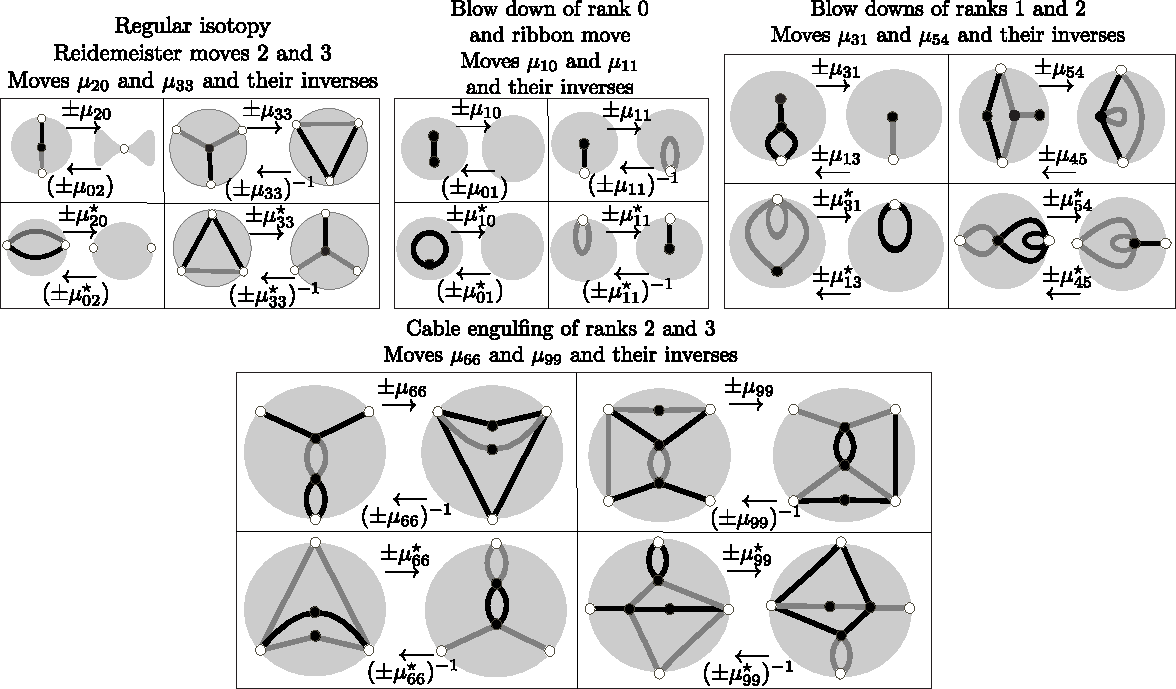
\includegraphics[width=16cm]{A.figs/blinkcalculus.pdf} 
  \end{center}
  \end{theorem}
 There are 64 local configurations divided into 32 pairs of left-right configurations.
 A move replaces the left (right) sub-blink of a pair by its right (left) counterpart.
 The exterior sub-blink to a fixed configuration is completely arbitrary, provided
 its intersection with the corresponding configurations are 
 the attachment vertices shown in the boundary of the shaded disk. These vertices
 are shown as shown as small white circles in the boundary of the shaded disk (or pinched disk
 in the case of $\rho_2$) wherem the configuration lies. 
 The number of such attachment vertices is the index of the 
 label for the move.



\section{Lickorish and moves by Kirby, Fenn-Rourke, Kauffman, Martelli}

A {\em knot} is an embedding of a circle, an $\mathbb{S}^1$, into $\mathbb{R}^3$ or  $\mathbb{S}^3$.
The {\em unknot} is a knot which is the boundary of a disk.
A {\em link with $k$ components} is an embedding of a disjoint union of $k$ copies of $\mathbb{S}^1$
into $\mathbb{R}^3$ or  $\mathbb{S}^3$. In this way, a knot is a link with one component.

Knots and links can be presented by their {\em decorated 
general position projections} into a fixed plane $\mathbb{R}^2$. {\em General position} means that 
in the image of the link there is no triple points and that at each neighborhood of
each double is the transversal crossing of two segments of the link, named {\em strands}. 
{\em Decorated} means that we keep the information
of which strand is the upper one, usually by removing a piece of the lower strand. In this paper
we use another way to decorate the link projections: the images of the link components are thich black curves
and the upper strands are indicated by a thinner white segment inside the thich black curve at the crossing.



In a grounding breaking work,  W.B.R. Lickorish in 1962, \cite{lickorish1962representation}, proved that
each closed orientable 3-manifold $\mathbb{M}^3$ can be encoded by a link in $\mathbb{S}^ 3$ 
where each one of its $k$ components
is endowed with an irreducible fraction (the framing) $\frac {\pm p}{q}$ 
where $q$ could be 0, and in the case $p$ must be 1 and the fraction
becomes $\pm \infty$. To construct the 3-manifold $\mathbb{M}^3$ 
from the framed link we act as follows: after removing from $\mathbb{M}^3$
an $\epsilon$-neighborhood $(\mathbb{S}^ 1 \times \mathbb{D}^2)_i$ of the $i$-th link we are left with 
$\mathbb{M}^ 3\backslash \bigcup_{i=1}^k (\mathbb{S}^ 1 \times \mathbb{D}^2)_i=
\mathbb{S}^ 3\backslash \bigcup_{i=1}^k (\mathbb{S}^ 1 \times \mathbb{D}^2)_i$. The fraction specifies, in the 
toroidal boundary inside $\mathbb{S}^ 3$, the homology type $(\pm p,q)$ of the curve that
is contractible in the solid torus inside $\mathbb{M}^3$. For each component, we then
identify the simple curve given by the homological base pair with the meridian of a canonical copy of a 
solid torus in $\mathbb{R}^ 3$  so as to completely specify the pasting of the solid torus 
closing the toroidal hole.
Lickorish's breakthrough was to prove that any $\mathbb{M}^3$ has inside it a finite number
$k$ of disjoint solid tori so that $\mathbb{M}^ 3\backslash \bigcup_{i=1}^k 
(\mathbb{S}^ 1 \times \mathbb{D}^2)_i=
\mathbb{S}^ 3\backslash \bigcup_{i=1}^k (\mathbb{S}^1 \times \mathbb{D}^2)_i$.
Actually, this result had been proved 2 years before 
by A. H. Wallace \cite{wallace1960modifications} by using differential geometry. However
it was the purely topological flavor of Lickorish's proof that spurs the subsequent developments.
  
In 1978 R. Kirby published his, to become famous, calculus of framed links, \cite{kirby1978calculus}.
The gist of this paper is that a finite number of two types of moves 
are enough to go from any framed
link inducing a closed oriented 3-manifold to any other such link inducing the same manifold.
One of the moves is absolutelly local: creating or cancellating a an unknot with frame in
$\{+1,-1,\infty,-\infty\}$. The other, {\em the band move} is non-local and infinite in number.
Shortly after in 1979 R. Fenn and C. Rourke (\cite{fenn1979kirby}) show that Kirby's moves could 
be replaced by an infinite number a single type of moves parametrized by $n$. This has been
a very useful reformulation with many applications, including Martelli's calculus (soon to be treated)
which uses it instead of the direct moves of Kirby.
 

In a recent paper B. Martelli \cite{martelli2012finite} presented a reformulation of
the Fenn-Rourke version (\cite{fenn1979kirby}) of Kirby's calculus \cite{kirby1978calculus}.
Our objective here is to further reformulate Martelli's moves so as to obtain a calculus
of blinks, which is an exact combinatorial counterpart for factorizing homeomorphisms of
closed orientable 3-manifolds. This goal is desirable because it has the consequence that each 3-manifold
become a subtle class of plane graphs. Our exposition is complete and elementary seeking
to reach both audiences: topologists and combinatorialists.



\begin{figure}[!h]
\begin{center}
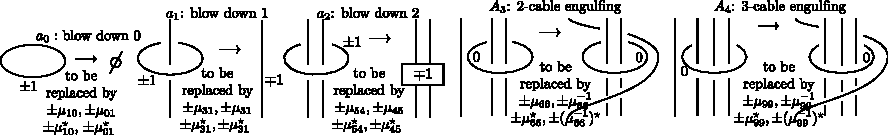
\includegraphics[width=16.5cm]{A.figs/Martelli.pdf} 
\caption{\sf Martelli's calculus on fractional framed links}
\label{fig:blinklinkgem}
\end{center}
\end{figure} 

\begin{figure}[!h]
\begin{center}
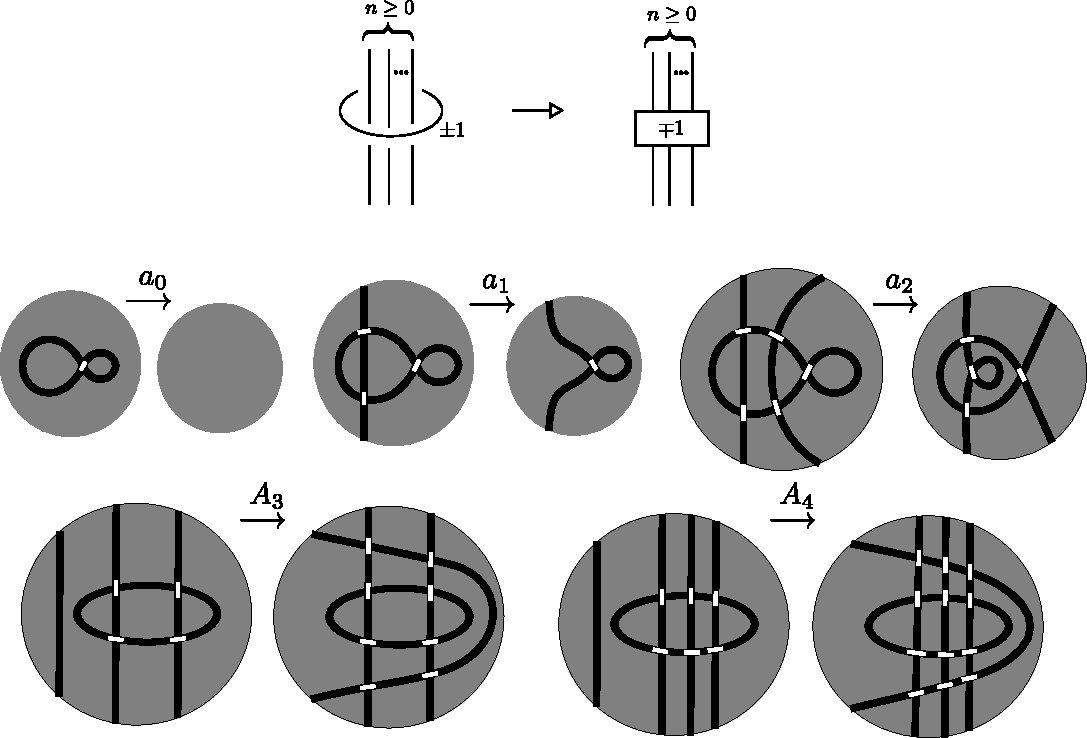
\includegraphics[width=13.5cm]{A.figs/FennRourkeMartelliBlackboard.pdf} 
\caption{\sf Fenn-Rourke infinite 1-parametrized blown-down moves 
and Martelli's moves in blackboard framed form}
\label{fig:FennRourkeMartelliBlackboard}
\end{center}
\end{figure} 


\section{Proof of the Theorem}

\begin{figure}[!h]
\begin{center}
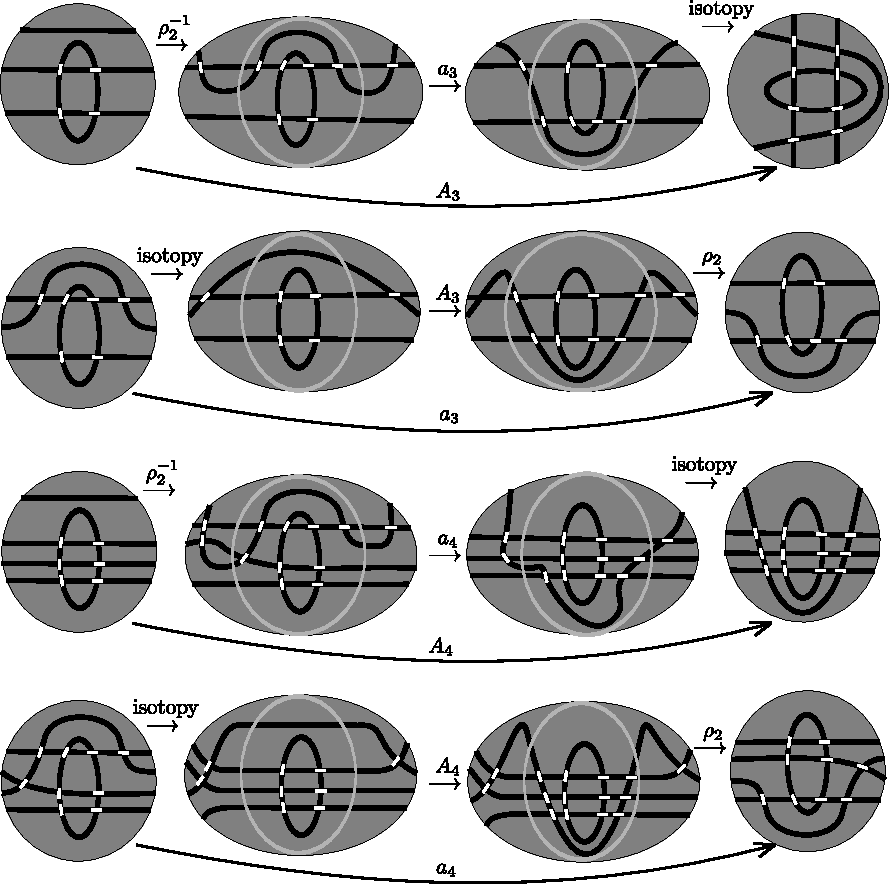
\includegraphics[width=14cm]{A.figs/proofequivalencea3A3a4A4.pdf} 
\caption{\sf A proof that in the presence of $\pm \rho_2^{\pm 1}$, $a_3 \equiv A_3$ and $a_4 \equiv A_4$ }
\label{fig:proofequivalencea3A3a4A4}
\end{center}
\end{figure} 
\begin{lemma}
 In the presence of  $\rho_2^{\pm 1}$, moves $\pm a_3$ and $\pm A_3$ are equivalent and so are
 $\pm a_4$ and $\pm A_4$.
\end{lemma}
\begin{proof}
 We refer to  Fig. \ref{fig:proofequivalencea3A3a4A4}. Its first line proves that $\pm a_3 \Rightarrow \pm A_3$.
 The second line proves that $\pm A_3 \Rightarrow \pm a_3$. The third line proves 
 that $\pm a_4 \Rightarrow \pm A_a$. The last line proves that $\pm A_4 \Rightarrow \pm a_4$. 
\end{proof}



\begin{figure}[!htb]
\begin{center}
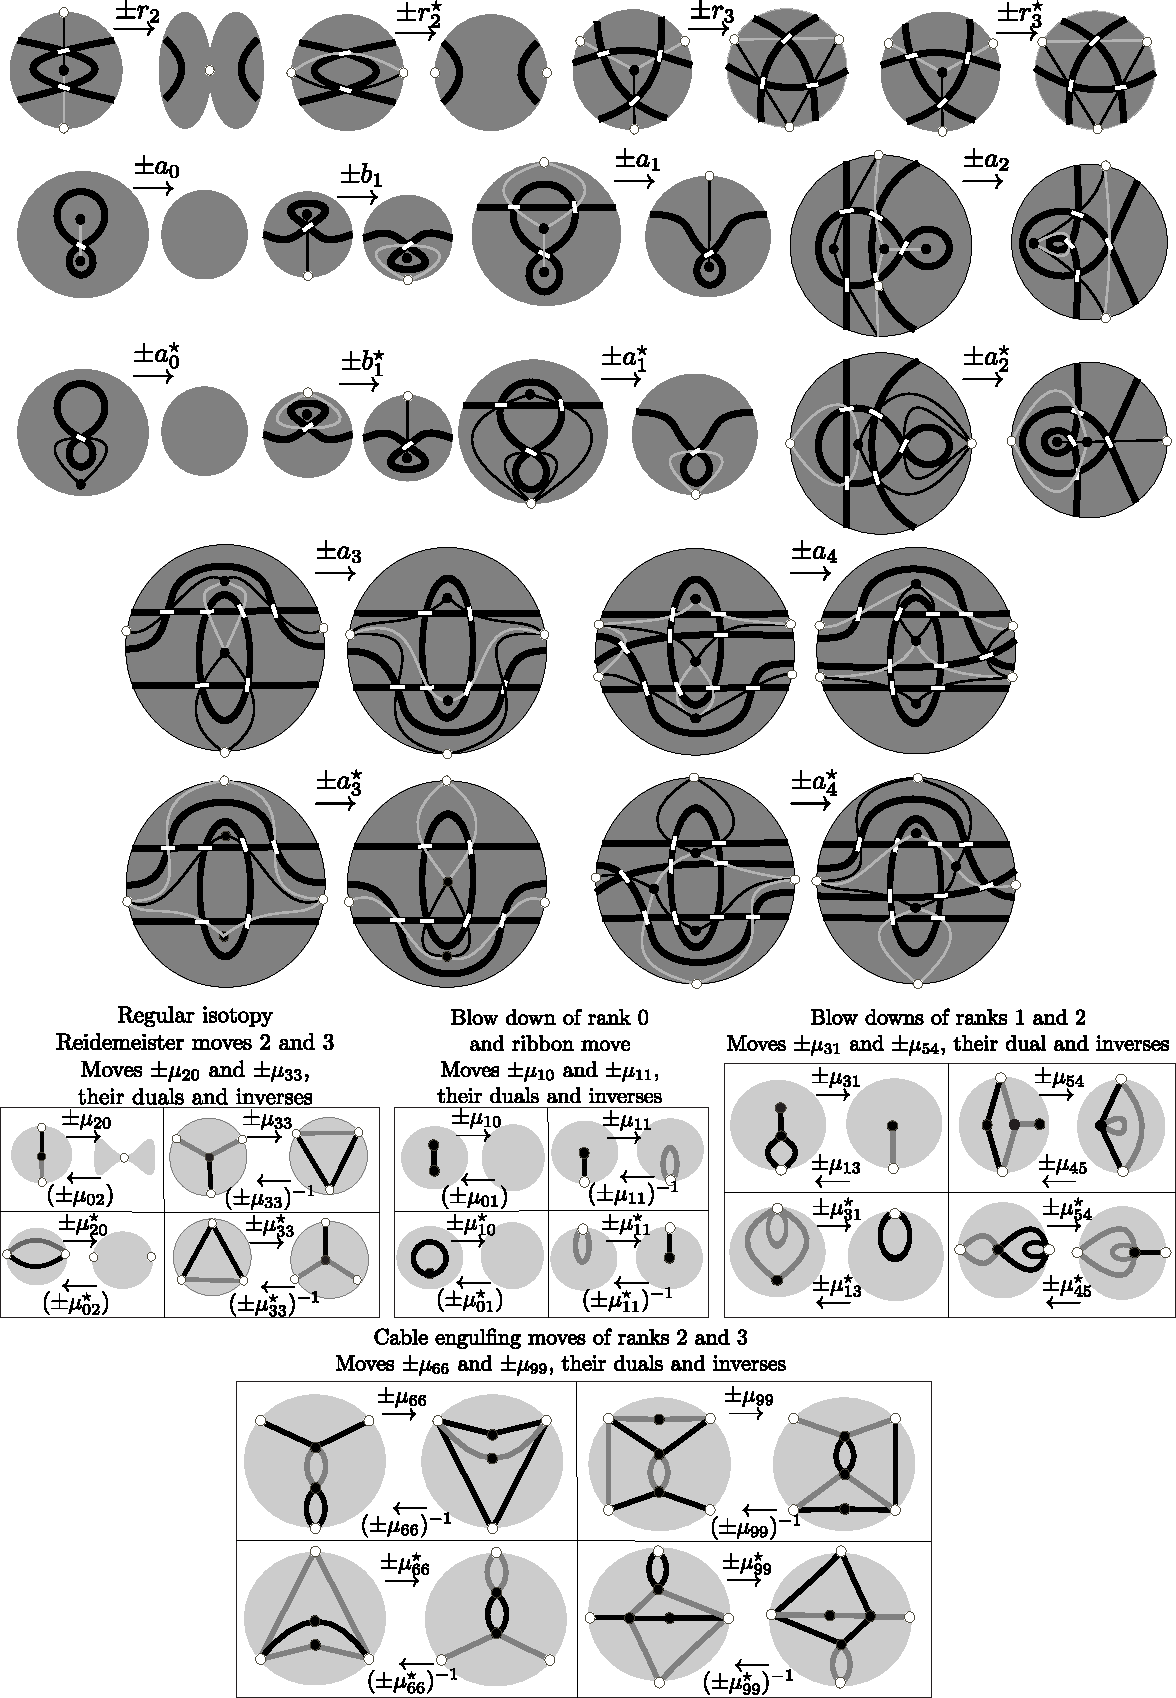
\includegraphics[scale=0.8]{A.figs/blinkandlinktogether.pdf}
\caption{Links \& blinks together implying moves for the blink calculus, concluding the proof of the Theorem 1.1}
\label{fig:blinkandlinktogether}
\end{center}
\end{figure}


% \begin{figure}[!h]
% \begin{center}
% \includegraphics[width=12.5cm]{A.figs/seconddoubtB.pdf}
% \caption{\sf Finding presentations for the fundamental groups of $M^ 3[2125]$ and $M^ 3[2165]$}
% \label{fig:seconddoubtB}
% \end{center}
% \end{figure}

%-----------------------------------
\bibliographystyle{plain}
%\bibliographystyle{is-alpha}
%\addcontentsline{toc}{bibliografia}{\MakeTextUppercase{Refer�ncias Bibliogr�ficas}}
%\bibliography{d:/slsl\3.DadosSostenes.35.ArtigosLivros.bibtexGoogleScholar/bibtexIndex.bib} % bib file is slsl.bib
%\bibliography{~/home/ricardo/Dropbox/35.ArtigosLivros.bibtexGoogleScholar/bibtexIndex.bib}
\bibliography{bibtexIndex.bib}
%\bibliography{slsl}


\vspace{5mm}
\begin{center}
\hspace{7mm}
\begin{tabular}{l}
   S\'ostenes L. Lins\\
   Centro de Inform\'atica, UFPE \\
   Av. Jornalista Anibal Fernandes s/n\\
   Recife, PE 50740-560 \\
   Brazil\\
   sostenes@cin.ufpe.br
\end{tabular}


\end{center}


\end{document}

\begin{figure}[!htb]
\begin{center}
\includegraphics[scale=0.8]{A.figs/seconddoubt.pdf}
\caption{Are these 3-manifolds homeomorphic?}
\label{fig:seconddoubt}
\end{center}
\end{figure}

% \printindex
